\documentclass[11pt, oneside]{article}   	% use "amsart" instead of "article" for AMSLaTeX format
\usepackage{geometry}                		% See geometry.pdf to learn the layout options. There are lots.
\geometry{letterpaper}                   		% ... or a4paper or a5paper or ... 
%\geometry{landscape}                		% Activate for for rotated page geometry
%\usepackage[parfill]{parskip}    		% Activate to begin paragraphs with an empty line rather than an indent
\usepackage{graphicx}				% Use pdf, png, jpg, or eps§ with pdflatex; use eps in DVI mode
								% TeX will automatically convert eps --> pdf in pdflatex		
\usepackage{amssymb}
\usepackage{amsmath}
\usepackage{parskip}
\usepackage{color}

\title{$\hat{\bf{n}} \ dS$ six ways}
%\author{The Author}
%\section{}
% \subsection*{R code}
\date{}							% Activate to display a given date or no date

\graphicspath{{/Users/telliott_admin/Dropbox/Tex/png/}}

% \begin{center} 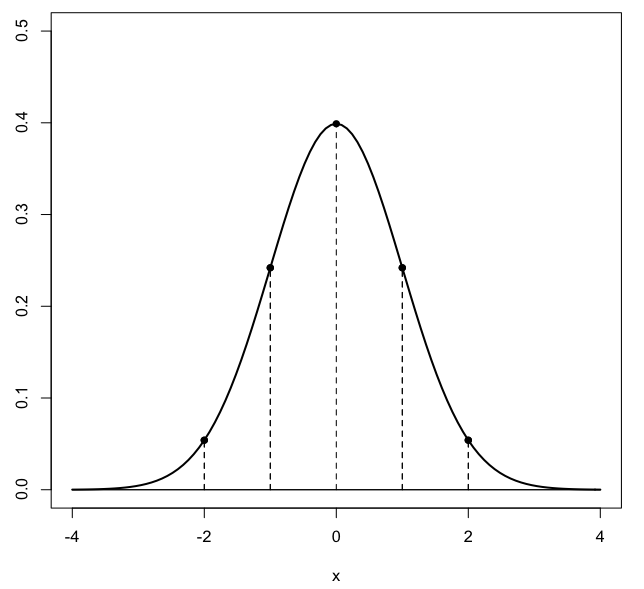
\includegraphics [scale=0.4] {gauss3.png} \end{center}
% \begin{bmatrix} a  &  b \\ c  &  d \end{bmatrix}
% \bigg |_

\begin{document}
\maketitle
\Large
%\noindent

\subsection*{plane}
In the $xy$-plane things are really easy.  The normal vector points straight up.  It is $\hat{\mathbf{k}}$ or
\[ \hat{\mathbf{n}} = \ <0,0,1> \]
Similarly, the surface element is just $dA$, so we have
\[ \hat{\mathbf{n}} \ dS = \ <0,0,1>  \ dx \ dy \]

\subsection*{cylinder}
On the surface of a cylinder the normal vector points straight out (no $z$ component).  If we look down from the top at the circular cross-section, the normal vector points out with components 
\[ \mathbf{n} = <x,y,0> \]
The length of $\mathbf{n}$ is $a$, the radius of the cylinder, so
\[ \hat{\mathbf{n}} = \frac{1}{a} \ <x,y,0> \]
The surface area element in the vertical direction is just $\Delta z$, while in the horizontal direction it is $r$ or $a$ times $\Delta \theta$, thus 
\[ \Delta S = a \ \Delta \theta \ \Delta z \]
\[ dS = a \ d \theta \ dz \]
\[ \hat{\mathbf{n}} \ dS = \ <x,y,0>  \ d \theta \ dz \]
Although it seems weird to mix $x,y$ with $\theta$, the idea is to keep things like this until we do the dot product with the field as will usually happen.

\subsection*{sphere}
On the surface of a sphere, the normal vector again points straight out.  It is
\[ \mathbf{n} = <x,y,z> \]
as we've seen before.  If the sphere has radius $a$, then the length of $\mathbf{n}$ is $a$, and
\[ \hat{\mathbf{n}} = \frac{1}{a} \ <x,y,z> \]
The surface of the sphere is parametrized by just $\phi$ and $\theta$ (no $r$ since it is fixed $r=a$).  Looking down at the horizontal circular cross-section for a given $\phi$, the radius of that circle is $a \sin \phi$, so the horizontal component of the surface area element is $a \sin \phi \ \Delta \theta$.  The vertical component is a great circle (radius $r = a$), so its length is just $a \ \Delta \phi$.

\[ \Delta S = a^2 \ \sin \phi \ \Delta \phi \ \Delta \theta \]
\[ dS = a^2 \ \sin \phi \ d \phi \ d \theta \]
Let's just check:
\[ \int dS = \int_0^{2 \pi} \int_0^{\pi} a^2 \ \sin \phi \ d \phi \ d \theta \]
\[ = 2 \pi a^2  \int_0^{\pi} \ \sin \phi \ d \phi \]
\[ = 2 \pi a^2 \ [ \ - \cos \phi  \ \bigg |_0^{\pi} \ ] \]
\[ = 4 \pi a^2 \]
and
\[ \hat{\mathbf{n}} \ dS = a \ <x,y,z>   \ \sin \phi \ d \phi \ d \theta \]

\subsection*{graph of a function}
If our surface is the graph of a function $g(x,y)$ then we can just remember the formula
\[ \hat{\mathbf{n}} \ dS = \ <-f_x,-f_y,1>  \ dx \ dy  \]
If we forget and need to work it out, the deal is that we get a linear approximation to the plane surface using $f_x$ and $f_y$ so that
\[ \mathbf{u} = <1,0,f_x> \ dx \]
\[ \mathbf{v} = <0,1,f_y> \ dy \]

The cross-product $\mathbf{u} \times \mathbf{v}$ gives 
\[ \mathbf{N} = \ <-f_x,-f_y,1>  \]
The length of $\mathbf{N} $ is
\[ |\mathbf{N}| = \sqrt{f_x^2 + f_y^2 + 1} \]
so 
\[ \hat{\mathbf{n}} = \frac{\mathbf{N}}{|\mathbf{N}|} = \ \frac{<-f_x,-f_y,1>}{\sqrt{f_x^2 + f_y^2 + 1}}  \]
However, $dS$ is larger than its shadow in the $xy$-plane by exactly this same factor
\[ dS \ \cos \theta = dA \]
where 
\[\cos \theta = \frac{\mathbf{n} \cdot \hat{\mathbf{k}} }{|\mathbf{n}| \ |\mathbf{k}|}=  \frac{1}{\sqrt{f_x^2 + f_y^2 + 1}} \]
Hence
\[ \hat{\mathbf{n}} \ dS =  \hat{\mathbf{n}} \ \frac{1}{\cos \theta} \ dA = \ \frac{<-f_x,-f_y,1>}{\sqrt{f_x^2 + f_y^2 + 1}} \ \sqrt{f_x^2 + f_y^2 + 1} \ dA \]
\[ = \ <-f_x,-f_y,1>  \ dA  \]
\[ = \ <-f_x,-f_y,1>  \ dx \ dy  \]
Depending on whether $\mathbf{n}$ points up or down we may change the sign.

\subsection*{parametrization (parameterization)}
More generally, we may have only a parametrization of the surface (it's not an explicit function $f(x,y)$).
\[ S =
\left\{
	\begin{array}{l}
		x  = x(u,v)  \\
		y  = y(u,v)  \\
		z  = z(u,v)
	\end{array}
\right.
\]
Then
\[ \hat{\mathbf{n}} \ dS = | \mathbf{r_u} \times \mathbf{r_v} | \ du \ dv \]

\subsection*{normal vector}
Auroux has a last example, in which we only know a normal vector $\mathbf{N}$ to the surface $S$.  Examples include a plane 
\[ ax + by + cz = d  \]
\[ \mathbf{N} = \ <a,b,c> \]
or $S$ is given by 
\[ g(x,y,z) = 0 \]
\[ \mathbf{N} = \nabla g \]
Then
\[ dS = \frac{1}{\cos \theta} \ dA = \frac{|\mathbf{N}|}{\mathbf{N} \cdot \hat{\mathbf{k}}} \ dA \]
\[ \hat{\mathbf{n}} \ dS  = \frac{|\mathbf{N}| \ \hat{\mathbf{n}}}{\mathbf{N} \cdot \hat{\mathbf{k}}} \ dA \]
As Auroux says, what happens if I take the unit normal $\mathbf{n}$, and I multiply it by the length of my other normal $|\mathbf{N}|$?  It's just $\mathbf{N}$.
\[ \hat{\mathbf{n}} \ dS  = \frac{\mathbf{N}}{\mathbf{N} \cdot \hat{\mathbf{k}}} \ dA \]
And again, this is "within sign", depending on how $\hat{\mathbf{n}}$ is oriented.



\end{document}  